\section*{Treść zadania}
\begin{enumerate}
    \item Zaprojektować licznik rewersyjny liczący w przód od 0..9 i w tył od 9..0 w kodzie (UZUPEŁNIJ). Licznik powinien zawierać:
    \begin{itemize}
        \item COUNTING DIRECTION (CD). Wartość logiczna 0 oznacza liczenie w przód.
        \item SET VALUE (SV). Sygnał nadrzędny asynchroniczny, który ustawia aktywne zero wartość licznika.
        \item CLOCK ENABLE (CE). Licznik liczy przy CE $ = 1$ i nie liczy przy CE $= 0$.
    \end{itemize}
    \item Przeprowadzić symulację układu, w której w formie sekwencyjnej pojawiają się zmiany sygnałów: \\
    Zegarowego, CE, CD, SV. Sprawdzić wszystkie funkcje licznika.
\end{enumerate}

\begin{figure}[!htb]
    \centering
    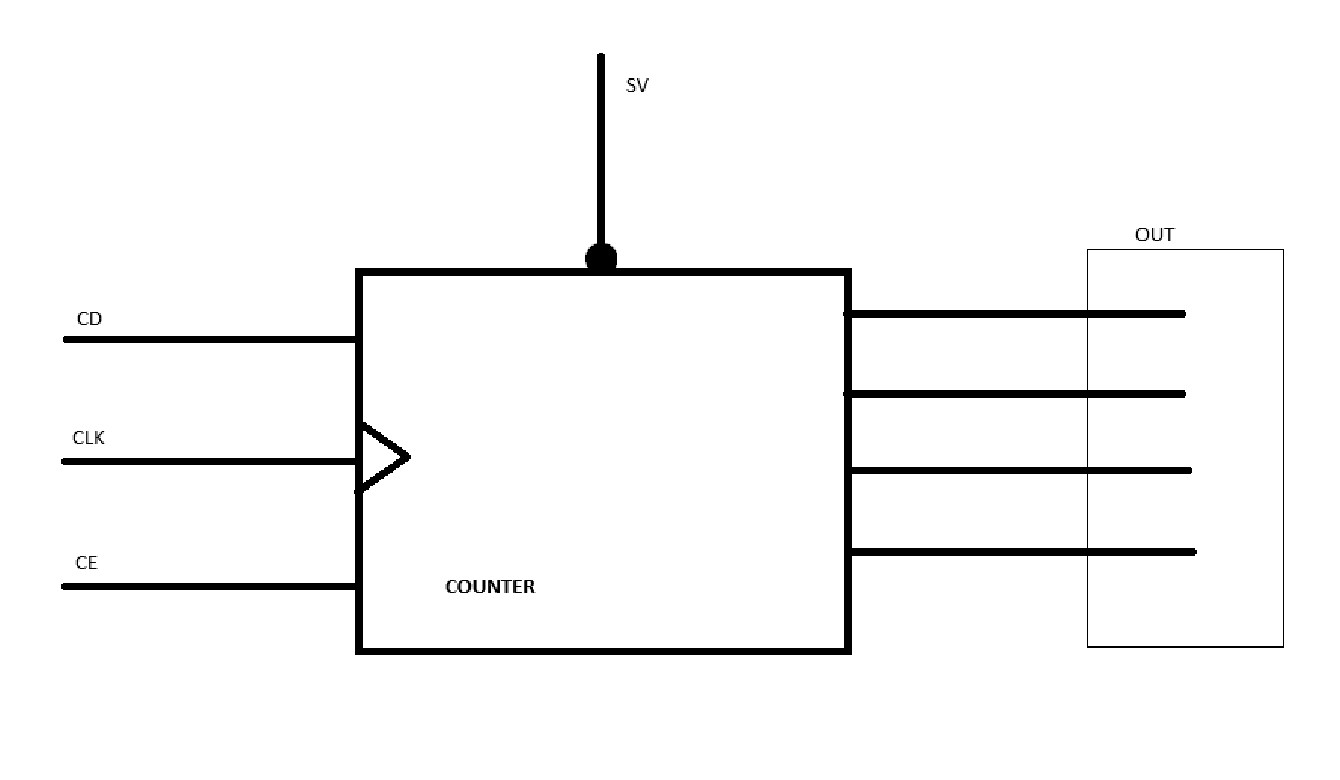
\includegraphics[height=10cm]{./images/Counter.jpg}
\end{figure}

\clearpage

\section{Kod Verilog}

\begin{lstlisting}

`timescale 1ns / 1ps


module main(
    input CLK,
	 input CE,
	 input CD,
	 input SV,
	 output [3:0] out
    );


reg [3:0] current_value;
reg [3:0] next_value;

initial
begin
	current_value = 4'b0000;
end


always @(posedge CLK or negedge SV)
begin
	if ( SV == 0) 
	begin
		if ( CD == 0 ) current_value = 4'b0000;
		else current_value = 4'b1111;
	end
	else if ( CE == 1 )	current_value = next_value;
end


always @ (current_value or CD)
begin
	if (CD == 0)
	begin
		case(current_value)
			4'b0000 : next_value = 4'b0001; //0 kod Aikena
			4'b0001 : next_value = 4'b0010; //1 
			4'b0010 : next_value = 4'b0011; //2
			4'b0011 : next_value = 4'b0100; //3
			4'b0100 : next_value = 4'b1011; //4
			4'b1011 : next_value = 4'b1100; //5
			4'b1100 : next_value = 4'b1101; //6
			4'b1101 : next_value = 4'b1110; //7
			4'b1110 : next_value = 4'b1111; //8
			4'b1111 : next_value = 4'b0000; //9
		endcase
	end
	else
	begin
		case(current_value)
			4'b0000 : next_value = 4'b1111; //0 kod Aikena
			4'b0001 : next_value = 4'b0000; //1 
			4'b0010 : next_value = 4'b0001; //2
			4'b0011 : next_value = 4'b0010; //3
			4'b0100 : next_value = 4'b0011; //4
			4'b1011 : next_value = 4'b0100; //5
			4'b1100 : next_value = 4'b1011; //6
			4'b1101 : next_value = 4'b1100; //7
			4'b1110 : next_value = 4'b1101; //8
			4'b1111 : next_value = 4'b1110; //9
		endcase
	end
end




assign out = current_value;

endmodule

\end{lstlisting}

\section{Kod w symulacji}

\begin{lstlisting}

	`timescale 1ns / 1ps

	module Sym1;
	
		// Inputs
		reg CLK;
		reg CE;
		reg CD;
		reg SV;
	
		// Outputs
		wire [3:0] out;
	
		// Instantiate the Unit Under Test (UUT)
		main uut (
			.CLK(CLK), 
			.CE(CE), 
			.CD(CD), 
			.SV(SV), 
			.out(out)
		);
		
		integer i;
		initial begin
			// Initialize Inputs
			CLK = 0;
			CE = 0;
			CD = 0;
			SV = 1;
	
			// Wait 100 ns for global reset to finish
			#50;
			
			//fork
			//begin
				CE = 1;
				for(i=0; i<11; i=i+1)
				begin
					#25 CLK = 1;
					#25 CLK = 0;
				end
			//end
				CE = 0;
				for(i=0; i<2; i=i+1)
				begin
					#25 CLK = 1;
					#25 CLK = 0;
				end
			
			#50;
			SV = 0;
			#50;
			SV = 1;
			//fork
			//begin
				CE = 1;
				for(i=0; i<11; i=i+1)
				begin
					#25 CLK = 1;
					#25 CLK = 0;
				end
			//end
				CE = 0;
				for(i=0; i<2; i=i+1)
				begin
					#25 CLK = 1;
					#25 CLK = 0;
				end
			
			CD = 1;
			
			#50;
			SV = 0;
			#50;
			SV = 1;
			
			CE = 1;
				for(i=0; i<11; i=i+1)
				begin
					#25 CLK = 1;
					#25 CLK = 0;
				end
			//end
				CE = 0;
				for(i=0; i<2; i=i+1)
				begin
					#25 CLK = 1;
					#25 CLK = 0;
				end
			
			#50;
			SV = 0;
			#50;
			SV = 1;
			//fork
			//begin
				CE = 1;
				for(i=0; i<11; i=i+1)
				begin
					#25 CLK = 1;
					#25 CLK = 0;
				end
			//end
				CE = 0;
				for(i=0; i<2; i=i+1)
				begin
					#25 CLK = 1;
					#25 CLK = 0;
				end
				
		end
	endmodule
	
	

\end{lstlisting}